\chapter{Algorithmic  composition}

\section{Historical framework}\label{historical-framework}

The first piece of music written by a computer is the \textit{Illiac Suite} for string quartet.

It was realized in 1956 at Illinois University.

Differently from music illustred in previous chapter computer did not generate the waveform but a symbolic representation of musical parameters to be transcribed into a musical score.

\begin{center}
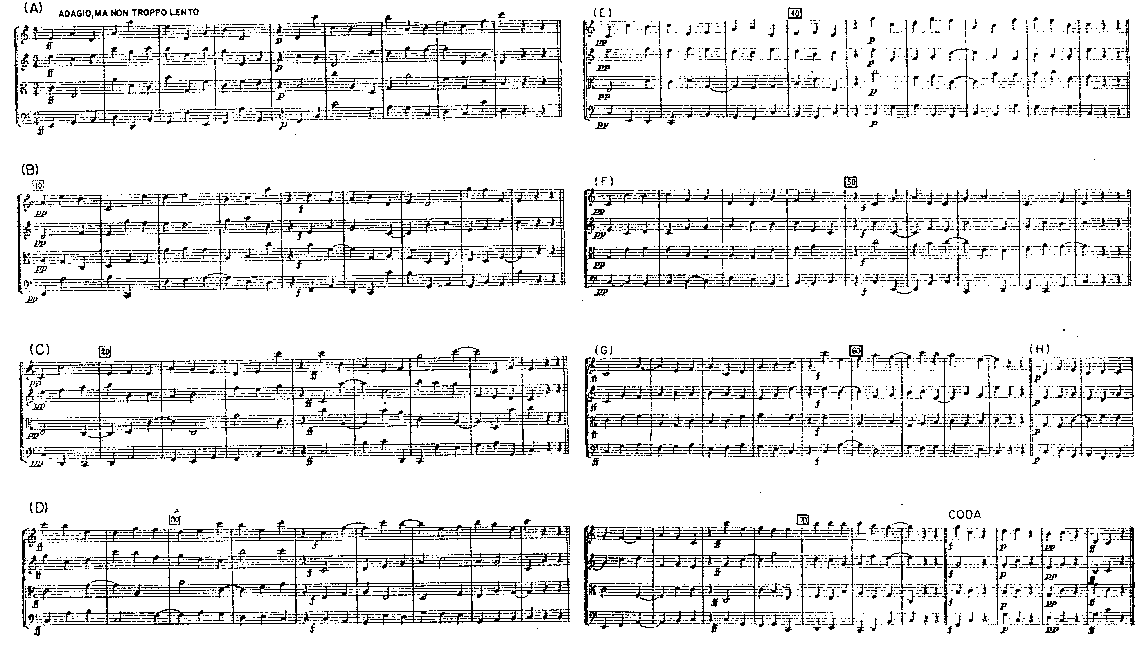
\includegraphics[scale=1]{../img/illiac.png}
\end{center}

This work was an experiment to test various algorithms for composition.

\begin{enumerate}
\def\labelenumi{\arabic{enumi}.}
\tightlist
\item random music \(\rightarrow\) no rules.
\item skip-stepwise rule \(\rightarrow\) no more than one repeated note.
\item cantus firmus starts on C with C chord for opening \(\rightarrow\) cadence on C with leading tone in one of the four voices \(\rightarrow\) resolution f tritone in VII-6, e.g.~F/B must resolve to E/C.
\item octave-range rule.
\item only consonant chords permitted except for 6-4 chords \(\rightarrow\) harmonic subroutine added.
\item parallel unisons, octaves, fifths and fourths still permitted \(\rightarrow\) melodic subroutine added.
\item parallel fourths, 6-4 chords containing tenth still permitted.
\item best counterpoint.
\end{enumerate}

Another important composer in the development of algorithmic music was the greek composer (naturalized french) Iannis Xenakis.

He used formulas developed by scientists to describe the behavior of particles in gases.

He saw his stochastic compositions as clouds of sound with individual notes as the analogue of gas particles organizing in this way clouds of notes.

The choice and distribution of notes was determined by procedures involving random choice, probability tables weighing the occurrence of specific events against those of others.


Iannis Xenakis - \href{http://www.musicaecodice.it/gitmedia/emc/5_media/xen1.mp4}{Pithoprakta} for Orchestra (1955-56) - extract.

Another composer involved in this fields was Gottfried Michael Koenig that worked at the Utrecht University Institute of Sonology and wrote about his Project 1 software:

\textit{Project 1 is based on the findings of serial composition technique, and aims at the experimental experience of chance-governed constellations of parameter values. Chance, in this instance, replaces the permutations to which the serial composer was accustomed to
subjecting rows, the consequences of which action for the resulting constellations of material was scarcely more predictable than in the case of aleatoric manipulations. Just as serial technique soon abandoned the''pointillist" style in order to apply the organizational principle to pre-formed units, ``groups'', the idea behind Project 1 likewise assumes that the unpredictability of chance will be neutralized by given
lists of material and the appropriate selection of items from the lists, in order to facilitate the formation of medium-sized and larger form categories.}

In more recent times and outside the academic environment a composer like Brian Eno writes:

\textit{Since I have always preferred making plans to executing them, I have
gravitated towards situations and systems that, once set into operation,
could create music with little or no intervention on my part. That is to
say, I tend towards the roles of planner and programmer, and then become
an audience to the results.}

Nowadays it is one of the most explored artistic fields in generative artificial intelligence.

\section{Software installation}\label{software-installation}

In addition to SuperCollider and sc\_kernel (optional) install: 

\begin{itemize}
\tightlist
\item \href{https://lilypond.org/}{Lilypond} 
\item \href{https://github.com/n-armstrong/fosc}{Fosc} (a Supercollider API for generating musical notation in lilypond)
\end{itemize}

Configure Fosc:

\begin{enumerate}
\def\labelenumi{\arabic{enumi}.}
\tightlist
\item download the zip file
\item rename the \textit{fosc-master} folder to \textit{fosc}.
\item select SuperCollider (base) Kernel in this notebook (optional).
\item find your SuperCollider user extension hidden folder path:

\begin{lstlisting}[frame=single] 
Platform.userExtensionDir
\end{lstlisting}

\item move the \textit{fosc} folder to your SuperCollider User Extensions folder.
\item search in SuperCollider Qarks \textit{wslib} and installi it.
\item recompile Class library in SuperCollider or Refresh SuperCollider Kernel in Notebook.
\item add code to allow Fosc to communicate with LilyPond to your sclang startup file.

\pagebreak

Mac users:

\begin{lstlisting}[frame=single] 
s.boot;

~lilypath="/Applications/lilypond-2.24.4/bin"; // Lilypond path
~filepath="/absolute/path/to/filename";        // without extension

Fosc.lilypondPath = ~lilypath++"/lilypond";
Fosc.lilypondVersion;

~print = {arg pitch, dur=[1/4], vel=[nil], tsig=[4,4], bpm=60, 
              filepath="/absolute/path/to/filename";
          var staff, mus, ts, seq, dn;
          
          Routine({        
          dur = dur.collect{arg i;
                      if(i.isSequenceableCollection)
                                {i[0]*i[1].normalizeSum}{i}}.flat;  
          mus = FoscLeafMaker().(pitches:pitch, durations:dur);
          dn = #['!','ppppp','pppp','ppp','pp','p','mp','mf',
                 'f','ff','fff','ffff','fffff'];
          mus.selectLeaves().do({arg item, id; 
                                 item.attach(FoscDynamic(
                                                i = vel.wrapAt(id);
                                                case
                                                {i==nil}{dn[0]}
                                                {i>=1 && i<=9}{dn[1]}
                                                {i>=10 && i<=19}{dn[2]}
                                                {i>=20 && i<=29}{dn[3]}
                                                {i>=30 && i<=39}{dn[4]}
                                                {i>=40 && i<=49}{dn[5]}
                                                {i>=50 && i<=59}{dn[6]}
                                                {i>=60 && i<=69}{dn[7]}
                                                {i>=70 && i<=79}{dn[8]}
                                                {i>=80 && i<=89}{dn[9]}
                                                {i>=90 && i<=99}{dn[10]}
                                                {i>=100 && i<=109}{dn[11]}
                                                {i>=110}{dn[12]} 
                                                )) 
                                 });
            staff = FoscStaff(mus);
            ts    = FoscTimeSignature(tsig);
            staff[0].attach(ts);
            staff.writePDF(filepath++".ly");
            
            seq = Pbind(
                      \midinote, Pseq(pitch.replace([nil],\rest),
                                   if(dur.size > pitch.size){inf}{1}),
                      \dur,      Pseq(dur * tsig[1],
                                   if(dur.size>pitch.size){1}{inf}),
                      \amp,      Pseq((vel.replace([nil],100)/127)**2,inf)
                        );
            ~midi = SimpleMIDIFile.new( filepath++'.mid' ); 
            ~midi.init;                  
            ~midi.init0(bpm,tsig[0].asString++"/"++tsig[1].asString);
            ~midi.timeMode = \ticks;   
            ~midi.fromPattern(seq);
            ~midi.checkWrite(filepath++'.mid', true);   
            1.wait;
            ~midi.play(TempoClock(bpm/60));
          }).play;
        };
\end{lstlisting}

\pagebreak

Windows users:

\begin{lstlisting}[frame=single] 
s.boot;

~lilypath="/absolute/path/to/lilypond-2.24.4/bin"; // Lilypond path
~filepath="/absolute/path/to/filename";            // without extension

Fosc.lilypondPath = ~lilypath++"/lilypond.exe";
Fosc.lilypondVersion;

~print = {arg pitch, dur=[1/4], vel=[nil], tsig=[4,4], bpm=60, 
              filepath="/absolute/path/to/filename"; 
          var staff, mus, ts, seq, dn;
          
          Routine({
          dur = dur.collect{arg i;
                       if(i.isSequenceableCollection)
                                {i[0]*i[1].normalizeSum}{i}}.flat;  
          mus = FoscLeafMaker().(pitches:pitch, durations:dur);
          dn = #['!','ppppp','pppp','ppp','pp','p','mp','mf',
                 'f','ff','fff','ffff','fffff'];
          mus.selectLeaves().do({arg item, id; 
                                 item.attach(FoscDynamic(
                                                i = vel.wrapAt(id);
                                                case
                                                {i==nil}{dn[0]}
                                                {i==0}{dn[0]}
                                                {i>=1 && i<=9}{dn[1]}
                                                {i>=10 && i<=19}{dn[2]}
                                                {i>=20 && i<=29}{dn[3]}
                                                {i>=30 && i<=39}{dn[4]}
                                                {i>=40 && i<=49}{dn[5]}
                                                {i>=50 && i<=59}{dn[6]}
                                                {i>=60 && i<=69}{dn[7]}
                                                {i>=70 && i<=79}{dn[8]}
                                                {i>=80 && i<=89}{dn[9]}
                                                {i>=90 && i<=99}{dn[10]}
                                                {i>=100 && i<=109}{dn[11]}
                                                {i>=110}{dn[12]}              
                                                ))
                                 });
            staff = FoscStaff(mus);
            ts    = FoscTimeSignature(tsig);
            staff[0].attach(ts);
            staff.writeLY(filepath++".ly");
("cd"+~lilypath+"&& lilypond -o"+filepath+filepath++".ly").unixCmd;
            seq = Pbind(
                      \midinote, Pseq(pitch.replace([nil],\rest),
                                      if(dur.size>pitch.size){inf}{1}),
                      \dur,      Pseq(dur * tsig[1],
                                      if(dur.size>pitch.size){1}{inf}),
                      \amp,      Pseq((vel.replace([nil],100)/127)**2,inf),
                        );
            ~midi = SimpleMIDIFile.new( filepath++'.mid' ); 
            ~midi.init;                  
            ~midi.init0(bpm,tsig[0].asString++"/"++tsig[1].asString);
            ~midi.timeMode = \ticks;   
            ~midi.fromPattern(seq);
            ~midi.checkWrite(filepath++'.mid', true); 
            1.wait;
            ~midi.play(TempoClock(bpm/60));
          }).play;  
        };
\end{lstlisting}

\item Test it - generates three files:

\begin{itemize}
\tightlist
\item test.ly
\item test.pdf
\item test.mid
\end{itemize}

We should also hear an audio preview with default intrumental timbre.

\begin{lstlisting}[frame=single] 
~bpm   = 60;
~tsig  = [3,4];
~pitch = [60,64,67,nil,67,64,72,[67,64],nil,64,60,[64,67,72]];
~durs  = [1/8];
~vels  = [nil];

~print.value(~pitch, dur:~durs, vel:~vels, tsig:~tsig, bpm:~bpm);
\end{lstlisting}
\end{enumerate}

We can load the midifile in an external midi sequencer or notation software as Musescore, Finale, Sibelius, etc.

\section{Symbolic musical representation and numbers}\label{symbolic-musical-representation-and-numbers}

The purpose of this computer music practice is to help the composer generate and manipulate musical elements according to the syntactic rules of their chosen musical language.

One of the goals of algorithmic composition or computer-aided composition is to translate numerical values \hspace{0pt}\hspace{0pt}into symbols specific to musical notation and vice versa.

The final result consists of a musical score that can be interpreted by human performers.

In computer music as well as in western musical tradition the following sound parameters are typically generated and/or manipulated:

\begin{itemize}
\tightlist
\item pitch (frequency).
\item rhythm (time).
\item dynamic (amplitude).
\item expression (timbre).
\end{itemize}

\subsection{Pitch}\label{pitch}

Some symbolic representations of frequency sorted by level of abstraction:

\begin{itemize}
\tightlist
\item note.
  \begin{itemize}
  \tightlist
  \item diatonic or chromatic representation by letters (notenames).
  \item fixed octave.
  \item relative to syntactically defined rules (western music tones, semitones).
  \item typically strings or chars data types.
  \end{itemize}

\begin{lstlisting}[frame=single] 
a = ['do', 're', 'mi', 'fa', 'sol', 'la', 'si', 'do']; // Note name
a = ['C3', 'D3', 'E3', 'F3',  'G3', 'A3', 'B3', 'C4']; // Octave
\end{lstlisting}

\item degree.

  \begin{itemize}
  \tightlist
  \item determine the pitch in degrees relative to a root note \(\rightarrow\) 0.
  \item no fixed octave.
  \item they may or may not be related to defined syntactic rules (scale degrees or other).
  \item typically int (positive and negative).
  \end{itemize}

\begin{lstlisting}[frame=single] 
a = [ 0, 2, 4, 5, 7, 9, 11, 12]; // Major scale model
a = [ -3, 5, 6, -4, 0, 2];       // A sequence 
\end{lstlisting}

\item note MIDI.
  \begin{itemize}
  \tightlist
  \item determines pitch as a fractional MIDI note.
  \item they are not related to syntactically defined rules.
  \item root note \(\rightarrow\) 60 = C4 = middle C.
  \item divided in semitones (int).
  \end{itemize}

\begin{lstlisting}[frame=single] 
a = [ 60, 62, 64, 65, 67, 69, 71, 72];
\end{lstlisting}

\item frequency.
  \begin{itemize}
  \tightlist
  \item determines the pitch as a frequency in Hertz (or cps).
  \item absolute values not relate in any way to syntactically defined rules.
  \item int or float
  \end{itemize}

\begin{lstlisting}[frame=single] 
a = [ 262, 294, 330, 349, 392, 440, 494, 523]; 
\end{lstlisting}
\end{itemize}

In computer music there are further forms of pitch representation but they can easily be traced back to those just mentioned.

In SuperCollider we can convert from a form to another:

\begin{lstlisting}[frame=single] 
~degree    = [0, 2, 4, 5, 7];   // Degree
~root      = 60;
~midinote  = root + a;          // Midi note   
~freqency  = ~midinote.midicps; // Frequency
~midinote1 = ~freqency.cpsmidi;
~degree1   = ~midinote1 - 60;

~midinote.postln;               // change
\end{lstlisting}

Chords \(\rightarrow\) 2D arrays.

\begin{lstlisting}[frame=single] 
a = [[60,64,67,72],62,[60,65,69,72],64,[62,65,67,71],62,[60,64,67,72]];
b = 1/4!6 ++ [1/2];

~print.value(a, b);
\end{lstlisting}

Rest \(\rightarrow\) nil instead note midi number.

\begin{lstlisting}[frame=single] 
a = [60,62,64,nil,65,67,nil,74,73,74,75,nil,76,72,nil,64];
b = [1/16];

~print.value(a, b);
\end{lstlisting}

\subsection{Rhythm}\label{rhythm}

We can define any kind of musical event in time choosing at least two of these parameters:

\begin{itemize}
\tightlist
\item onsets \(\rightarrow\) absolute time of a sound event relative to the beginning (as in DAW software).
\item delta times \(\rightarrow\) time between two consecutive sound events.
\item durations \(\rightarrow\) duration of a sound event.
\end{itemize}

All these parameters can be specified as:

\begin{itemize}
\tightlist
\item absolute measurement units (typicalli seconds or millisecond).
\item relative to a bpm.

  \begin{itemize}
  \tightlist
  \item 1 \(\rightarrow\) beat, reference unit (could be quarter, eight, whole, etc).
  \item 1/4 \(\rightarrow\) fractional notation.
  \item 0.5 \(\rightarrow\) multiply factor (result from fractional notation).
  \item 3:2 \(\rightarrow\) Rhythmic proportions (ratios of one single beat or its subdivisions).
  \end{itemize}
\end{itemize}

We can convert the values by simple mathematical operations.

\begin{lstlisting}[frame=single] 
~bpm = 82;
~sec = 60/~bpm;  // bpm     --> seconds
~bpm = 60/~sec;  // seconds --> bpm          
\end{lstlisting}

In the next paragraph we adopt the fractional notation as input (but inside it's converted to multiply facors of unit).

\begin{lstlisting}[frame=single] 
a = [72,76];
b = [1/16, 1/16, 1/8, 1/16, 1/16, 1/16, 1/16, 1/4,1/4];

~print.value(a, b);
\end{lstlisting}

If we want to define dotted or irregular rhythms we must use this syntax:

\begin{lstlisting}[frame=single] 
//    [unity, [subdivisions] ]
a = [ [1/4,   [3, 1        ] ] ];
\end{lstlisting}

\subsection{Dynamic}\label{dynamic}

Three different measurament units:

\begin{itemize}
\tightlist
\item 1.0 \(\rightarrow\) linear amplitude (floating point form 0.0 to 1.0).
\item 127 \(\rightarrow\) midi velocity (integer from 0 to 127).
\item -6 \(\rightarrow\) decibels (from -inf to 0.0).
\end{itemize}

Conversions:

\begin{lstlisting}[frame=single] 
~lin  = 64  / 127;  // velocity to linear
~vel  = 0.5 * 127;  // linear to velocity
~lin1 = -6.dbamp;   // dB to linear
~db   = 0.5.ampdb;  // linear to dB
~cub  = 0.5**4;     // linear to quartic (best for human perception)             
\end{lstlisting}

\subsection{Collections}\label{collections}

As we saw we can describe sets of values \hspace{0pt}\hspace{0pt}as
collections (arrays and lists).

Collections are a musically neutral data type as they can contain any
data type.

In algorithmic composition we can think it musically in two ways:

\begin{itemize}
\tightlist
\item out of time (pre compositional materials).
  \begin{itemize}
  \tightlist
  \item rules paradigm.
  \item item positions on x axis are indexes without time references (degree or other).
  \item scale
\begin{lstlisting}[frame=single] 
//          0   1   2   3   4   5   6   7         // Scale degrees
~dorico = [60, 62, 64, 65, 67, 69, 71, 72];       // Absolute pitches
~chrom  = [0, 1, 2, 3, 4, 5, 6, 7, 8, 9, 10, 11]; // Intervals
~durs   = [1/8];

~print.value(~dorico, ~durs);
\end{lstlisting}

  \item series
\begin{lstlisting}[frame=single] 
~serie  = [1, 10, 6, 4, 8, 2, 9, 7, 0, 5, 11, 3]; // Dodecaphony
~reich  = [64, 66, 71, 72, 73, 66];               // Minimalism
~durs   = [1/8];

~print.value(~reich, ~durs);
\end{lstlisting}

  \item harmonic fields (Array or Array 2D)
\begin{lstlisting}[frame=single]
~mayor = [0, 4, 7, 12];
~harm  = [[60, 64, 67, 72], [62, 65, 67, 71], [60, 65, 69,72], [60, 64, 69,72]];
~harmd = [[0, 4, 7, 12],  [2, 5, 7, 11],  [0, 5, 9,12], [0, 4, 9,12]];
~durs  = [1/8];

~print.value(~harm, ~durs);
\end{lstlisting}
  \end{itemize}
  
\item timeline.

  \begin{itemize}
  \tightlist
  \item sequence paradigm.
  \item items are placed on a timeline (x axis).
  \end{itemize}

\begin{lstlisting}[frame=single] 
//   - Sequence of index from defined scale
//          0   1   2   3   4   5   6   7
~scale  = [60, 62, 64, 65, 67, 69, 71, 72];      
~melody = 10.collect({rrand(0,7)});
~seq    = ~melody.collect({arg i; ~scale[i]});
                
~durs   = ([1/16,1/8,1/16]!3++[1/4]).flat; 

~print.value(~seq,~durs); 
\end{lstlisting}
\end{itemize}

\subsection{Live}\label{live}

Send numerical data via MIDI to external sound generators (Reaktor, GarageBand, Finale, Logic) without print it in a musical score.

Open a midi sound generator software and set it.

\begin{lstlisting}[frame=single, caption=Live midi out sender model] 
// 1. Checks which available MIDI sources and destinations there are, and
//    opens as many connections as desired

MIDIClient.init;

// 2. Choose the destination where you want send your MIDI data (id from 0)

c = MIDIOut.new(0); // 0 = "Driver IAC"
c.latency_(0);      // Set latency to 0 sec

// 3. Open an external MIDI sound bank (Reaktor, GarageBand, Finale, Logic)
// 4. Send some MIDI data.

~bpm   = 60;  
~note  = 100;     
~tsig  = [4,4];
~pitch = ~note.collect({rrand(60,75)});
~durs  = ~note.collect({[1/32, 1/32,1/32, 1/32,1/32,1/8, 1/16].choose});
~vels  = ~note.collect({[100, 40, 60].choose});
p = Pbind(
        \type, \midi,
        \midicmd, \noteOn,
        \midiout, c,
        \chan, 0,
        \midinote, Pseq(~pitch.replace([nil],\rest)),
        \sustain,  Pseq(~durs * ~tsig[1],inf),   // Duration
        \dur,  Pseq(~durs * ~tsig[1],inf),       // Delta time
        \amp, Pseq(~vels/127,inf),               // 0.0 to 1.0
        ).play;
\end{lstlisting}

\section{Generative techniques and processes}\label{generative-techniques-and-processes}

In western musical tradition superposition of two or more voices have only two approaches: 

\begin{itemize}
\tightlist
\item \href{http://www.musicaecodice.it/gitmedia/emc/5_media/palestrina1.mp4}{counterpoint} (horizontal dimension - static voice allocation).
\item \href{http://www.musicaecodice.it/gitmedia/emc/5_media/beetho1.mp4}{counterpoint} (harmony).
\end{itemize}

Approaches to which different musical languages refer.

We are going to explore compositional practices about them through three case studies:

\begin{itemize}
\tightlist
\item modes and scales (counterpoint).
\item harmonic fields (harmony).
\item XIX sec.~music (both).
\end{itemize}

In general if we want formalize our musical ideas we should act as in previous chapters.

Recap.

\begin{enumerate}
\def\labelenumi{\arabic{enumi}.}
\tightlist
\item define a set of parametric structures that we want to use as basic material according to musical rules (scale, modes, serie, chords, rhythmic or dynamic patterns, etc.).
\item define a set of possible modifications always starting from musical needs and rules (variations, filters, interpolations, augmentations, diminutions, etc.).
\item organize them over time by defining a formal structure choosing from two strategies:
  \begin{itemize}
  \tightlist
  \item top to bottom (from a fixed general structure to particular).
  \item bottom to top (from particular to a general formal structure).
  \end{itemize}
\end{enumerate}

In carrying out these three steps, we have only two possible approaches often mixed toghether:

\begin{itemize}
\tightlist
\item nondeterministic.
\item deterministic.
\end{itemize}

\subsection{Modes and scales}\label{modes-and-scales}

Both are based on the concept of \textit{mode} (gregorian and nedieval music) or \textit{scale} (baroque and classical music).

It define the interval patterns through which composer organize the pitches of a piece.

They are usually some kind of subdivision of the octave interval.

We can define it in interval or grades.

\begin{lstlisting}[frame=single] 
~major = [0,2,4,5,7,9,11,12]; 
\end{lstlisting}

Then we have to define a root note in midi values which will assume the function of the first degree (0)

\begin{itemize}
\tightlist
\item in modal rules is called \textit{finalis}.
\item in tonal (harmonic) rules is the \textit{tonality} (D major, E-flat minor, etc.).
\end{itemize}

\begin{lstlisting}[frame=single] 
~major = [0,2,4,5,7,9,11,12];  // Try to change intervals
~root  = 60;
~pitch = ~root + ~major;
~dur   = [1/8];

~print.value(~pitch, ~dur, filepath:~filepath); 
\end{lstlisting}

We can use historical models or invent our own.

\subsubsection{Scale}\label{scale}

In SuperCollider there is a Class that represent a repository of different scales from different coltures.

\begin{lstlisting}[frame=single] 
Scale.directory;
\end{lstlisting}

We can choose a scale from the available scales and then recall the interval model.

\begin{lstlisting}[frame=single] 
~model  = Scale.lydian;    // Try to change scale
~degree = ~model.degrees; 
~root   = 60;
~pitch  = ~root + ~degree ++[72];
~dur    = [1/8];

~print.value(~pitch, ~dur, filepath:~filepath); 
\end{lstlisting}

Once the interval model has been established, we can create a melody by recalling the different degrees of the model according to deterministic or indeterministic principles.

\subsubsection{Incises and sequences}\label{incises-and-sequences}

Define a function that generate a melodic cell (inciso) according to few simply rules:

\begin{enumerate}
\def\labelenumi{\arabic{enumi}.}
\tightlist
\item set the number of notes in the inciso (random from 5 to 7).
\item set a percentage of random rest in the inciso (from 0.0 to 1.0).

\begin{lstlisting}[frame=single] 
~model  = Scale.lydian.degrees; 
~inciso = {arg degrees=a, root=60, rrest=0.0;
           var notes, rests, pitch;
                notes = rrand(3,6);
                rests = [degrees,[nil]];      // [[degrees],[nil]]
                pitch = notes.collect{var i; 
                               i = rests.wchoose([1-rrest,rrest]).choose;
                               if(i.notNil){i = i + root} };
                pitch};

a = ~inciso.value(~model,rrest:0.2);
a.postln;
~print.value(a,[1/8])
\end{lstlisting}

\item set a percentage of random velocities to apply only on notes.
  \begin{itemize}
  \tightlist
  \item veld \(\rightarrow\) array from wich velocities are chosen.
  \item rvels \(\rightarrow\) percentage of vels (0.0-1.0).
  \end{itemize}

  N.B. Dynamic mark change only the note, if not specified is \textit{mezzoforte} (default).

\begin{lstlisting}[frame=single] 
~model  = Scale.lydian.degrees; 
~inciso  = {arg degrees=a, root=60, rrest=0.0, vels=[nil], rvels=0.0;
            var notes, rests, pitch, vel;
                notes = rrand(3,6);
                rests = [degrees,[nil]];      // [[degrees],[nil]]
                pitch = notes.collect{var i; 
                               i = rests.wchoose([1-rrest,rrest]).choose;
                               if(i.notNil){i = i + root} };
                vel = pitch.collect{arg i;
   if(i.notNil){[vels,[nil]].wchoose([rvels,1-rvels]).choose} }.flat;
                [pitch, vel]};

a = ~inciso.value(~model,rrest:0.2,vels:[30,100],rvels:0.7 );

~print.value(a[0],vel:a[1])
\end{lstlisting}

\item set a database of rhythmic patterns from which to extract one according to the number of pitches. Each pattern should be of the same lenght (a beat or its multiple).

\begin{lstlisting}[frame=single] 
~model  = Scale.lydian.degrees; 

~inciso =  {arg degrees=a, root=60, rrest=0.0, vels=[nil], rvels=0.0;
            var notes, rests, pitch, vel, rhytm;
                notes = rrand(3,6);
                rests = [degrees,[nil]];      // [[degrees],[nil]]
                pitch = notes.collect{var i; 
                        i = rests.wchoose([1-rrest,rrest]).choose;
                        if(i.notNil){i = i + root}
                                    };
                vel = pitch.collect{arg i;
        if(i.notNil){[vels,[nil]].wchoose([rvels,1-rvels]).choose} }.flat;
                switch(notes,
                    3, {rhytm = [   
                        [1/8,1/16,1/16],   // all in 1/4 or multiply
                        [1/16,1/8,1/16],       // 1 beats
                        [1/16,1/16,1/8],       // 1 beats
                        [1/4,[1/4,[3,1]]],     // 2 beats
                        [1/8, [1/8,[1,2]]]     // 1 beats
                                ].choose},
                    4, {rhytm = [   
                        [1/8,1/16,1/16,1/4],   // 2 beats
                        [1/4,1/16,1/8,1/16],   // 2 beats
                        [1/16, 1/4, 1/16,1/8], // 2 beats
                        [1/4,[1/4,[3, 1, 2]]], // 2 beats
                        [1/8,[1/8,[1, 1, 1]]]  // 1 beats
                                ].choose},
                    5, {rhytm = [   
                        [1/8,1/16,1/16,1/8,1/8],    // 2 beats
                        [1/8,1/16,1/8,1/16,1/8],    // 2 beats
                        [1/32, 1/4, 1/32,1/8,1/16], // 2 beats
                        [1/4,[1/4,[1, 2, 1, 1]]],   // 2 beats
                        [1/8,1/4, [1/8,[1, 1, 1]]]  // 2 beats
                                ].choose},
                    6, {rhytm = [   
                        [1/8,1/16,1/16,1/16,1/8,1/16],    // 2 beats
                        [1/8,1/32,1/8,1/32,1/8,1/16],     // 2 beats
                        [1/32, 1/8, 1/32, 1/8, 1/16,1/8], // 2 beats
                        [1/8,[1/4,[1, 2, 1, 1]], 1/8],    // 2 beats
                        [1/8,1/4, [1/8,[1, 1, 1]],1/8]    // 2 beats
                                ].choose};
                        );   
            [pitch, rhytm, vel]
            };

a = ~inciso.value(~model, rrest:0.2, vels:[20,100], rvels:0.2);
a[0].postln;
a[1].postln;
a[2].postln;
~print.value(a[0], a[1],a[2])
\end{lstlisting}

We can now construct several incises.

\begin{lstlisting}[frame=single] 
a = ~inciso.value(~model,rrest:0.2,vels:[20,100],rvels:0.3);
b = ~inciso.value(~model,rrest:0.3,vels:[20,100],rvels:0.3);

~pseq = (a[0] ++ b[0] ++ a[0]).flat;
~rseq = (a[1] ++ b[1] ++ a[1]).flatten(-1);
~vseq = (a[2] ++ b[2] ++ a[2]).flat;

~print.value(~pseq, ~rseq, vel:~vseq);
\end{lstlisting}

And concatenate them into a sequence.

\begin{lstlisting}[frame=single] 
a = ~pseq ++ ~pseq ++ ~pseq;
b = ~rseq ++ ~rseq ++ ~rseq;
c = ~vseq ++ ~vseq ++ ~vseq; 

~print.value(a, b, vel:c);
\end{lstlisting}
\end{enumerate}

\subsubsection{Melodic variations}\label{melodic-variations}

Bla bla bal

\subsubsection{Rhytmic variations}\label{rhytmic-variations}

Bla bla bal

\subsubsection{Accents}\label{accents}

Bla bla bal

\subsection{Harmonic fields}\label{harmonic-fields}

Bla bla bal

\subsection{XIX sec.~music}\label{xix-sec.-music}

Bla bla bal

\section{Composition sketches proposal}\label{composition-sketches-proposal}


